\section{Data Previews and Data Release 1} 
\label{sec:datapreview}

A series of three Data Previews (DP) and one Data Release (DR) are planned to support the community as they develop their LSST analysis software and workflows, and to enable high-impact science as soon as possible.
\begin{itemize}
\item Data Preview 0 (DP0): Based on simulated LSST-like data.
\item Data Preview 1 (DP1): Based on a subset of early science-grade commissioning data taken with either ComCam or LSSTCam.
\item Data Preview 2 (DP2): Based on a full reprocessing of all science-grade LSSTCam data taken during commissioning.
\item Data Release 1 (DR1): Based on the first six months of LSST data. 
\end{itemize}
Due to the relatively short time periods available for commissioning observations (\S~\ref{ssec:transition}), the Data Previews will necessarily be limited in their area and temporal coverage relative to a full Data Release. 

The data products that comprise the Data Previews and Data Releases are produced by the LSST Science Pipelines \citep{2019ASPC..523..521B,2018PASJ...70S...5B}.
For an introduction to the LSST data products, see \citet{RubinDataProductsAbridged} and for a detailed description, see the LSST \dpdd{},  \citedsp{LSE-163}.
Each Data Preview and LSST Data Release will be accompanied by its own release-specific DPDD\footnote{For an example data release DPDD, see the online DP0.2 documentation {\url{https://dp0-2.lsst.io/data-products-dp0-2/}}.}, giving e.g. the  database schema for the catalogs included in that dataset.
Table~\ref{tab:data-preview-summary} provides a summary of the expected early science data products available in DP0, DP1, DP2 and the LSST Data Release 1.
All LSST data products will be subject to the embargo periods described in  \citeds{DMTN-199}; 30 days during commissioning and 80 hours during operations for pixel data.

\begin{table}
\centering
\fontsize{6}{10}\selectfont 
\setlength{\tabcolsep}{6pt} % Default value: 6pt
{\renewcommand{\arraystretch}{1.2}
\begin{tabular}{|l|c|c|c|c|c|c|c|c|}
    \hline
\multicolumn{9}{|l|}{{\fontsize{9}{12}\selectfont \color{RubinDarkTeal}\textbf{Rubin Early Science Data Release Scenario}}}  \\\hline\hline
\multirow{2}{*} {} & 
        \tiny Jun 2021 & \tiny Jun 2022 & \tiny Jun 2023  & 
        \tiny \makecell{Oct 2024 -- \\ Jul 2025}  & 
        \tiny \makecell{ Nov 2025 -- \\ May 2026} & 
        \tiny \makecell{ May 2026 -- \\ Jan 2027} & 
        \tiny \makecell{ May 2027 -- \\ Jan 2028} & 
        \tiny \makecell{ May 2028 -- \\ Nov 2028} 
    \\ \cline{2-9}
        
        & \textbf{DP0.1}     &  \textbf{DP0.2}     &  \textbf{DP0.3}     &  \textbf{DP1}     &  \textbf{DP2}  &  \textbf{DR1} &  \textbf{DR2}  & \textbf{DR3} 
   \\\cline{2-9} 
       \multirow{3}{*}{\parbox{0.2\linewidth}{\vspace{0.5cm} \textbf{Data Product}}}  &   
        \rotatebox[origin=c]{90}{\tiny \makecell{ \textbf{DC2 Simulated} \\ \textbf{Sky Survey} }}  & 
        \rotatebox[origin=c]{90}{\tiny\makecell{\textbf{Reprocessed} \\ \textbf{DC2 Survey} }} &
	\rotatebox[origin=c]{90}{\tiny\makecell{\textbf{Solar System} \\ \textbf{PPDB}  \\ \textbf{Simulation}}}  &  
	\rotatebox[origin=c]{90}{\tiny\makecell{\textbf{ComCam or} \\ \textbf{ early} \\ \textbf{ LSSTCam} \\ \textbf{Data}}} & 
	\rotatebox[origin=c]{90}{\tiny\makecell{\textbf{LSSTCam} \\ \textbf{ Science} \\ \textbf{Validation}  \\ \textbf{Data}}} & 
	\rotatebox[origin=c]{90}{\tiny\makecell{\textbf{LSST First 6} \\ \textbf{ Months}  \\ \textbf{Data}}} &
	\rotatebox[origin=c]{90}{\tiny\makecell{\textbf{LSST Year 1} \\ \textbf{  Data}}} & 
	\rotatebox[origin=c]{90}{\tiny\makecell{\textbf{LSST Year 2} \\ \textbf{  Data}}} 
    \\\cline{2-9 } \hline
    
Raw Images   &   \mycirc[RubinDarkTeal]  &   \mycirc[RubinDarkTeal]  &    --  &   \mycirc[RubinDarkTeal]  &    \mycirc[RubinDarkTeal]  &    \mycirc[RubinDarkTeal]  &  \mycirc[RubinDarkTeal]  &    \mycirc[RubinDarkTeal]  \\  \arrayrulecolor{gray}\hline
DRP Processed Visit Images and Visit Catalogs         &    \mycirc[RubinDarkTeal]  &   \mycirc[RubinDarkTeal]  &    --  &   \mycirc[RubinDarkTeal]  &    \mycirc[RubinDarkTeal]  &    \mycirc[RubinDarkTeal]  &  \mycirc[RubinDarkTeal]    &    \mycirc[RubinDarkTeal]  \\\hline 
DRP Coadded Images      &   \mycirc[RubinDarkTeal]  &   \mycirc[RubinDarkTeal]  &    --  &   --  &    \mycirc[RubinDarkTeal]  &    \mycirc[RubinDarkTeal]  &  \mycirc[RubinDarkTeal]  &    \mycirc[RubinDarkTeal]  \\\hline
Object and ForcedSource Catalogs      &   \mycirc[RubinDarkTeal]  &   \mycirc[RubinDarkTeal]  &    --  &   --  &    \mycirc[RubinDarkTeal]  &    \mycirc[RubinDarkTeal]  &  \mycirc[RubinDarkTeal]  &   \mycirc[RubinDarkTeal]  \\ \hline
DRP Difference Images and DIASources       &  --  &   \mycirc[RubinDarkTeal]  &    --  &   --  &    \mycirc[RubinDarkTeal]  &    \mycirc[RubinDarkTeal]  &  \mycirc[RubinDarkTeal]  &    \mycirc[RubinDarkTeal]  \\  \hline
DRP ForcedSource Catalogs including DIA output     &  --  &   \mycirc[RubinDarkTeal]  &    --  &   --  &    \mycirc[RubinDarkTeal]  &    \mycirc[RubinDarkTeal]  &  \mycirc[RubinDarkTeal]  &    \mycirc[RubinDarkTeal]  \\  \hline
PP Processed Visit Images     & --  &   --  &    --  &   --  &    --  &    \mycirc[RubinDarkTeal]  &  \mycirc[RubinDarkTeal]   &    \mycirc[RubinDarkTeal]   \\ \hline 
PP Difference Images     & --  &   --  &    --  &   --  &    --  &    \mycirc[RubinDarkTeal]  &  \mycirc[RubinDarkTeal]   &    \mycirc[RubinDarkTeal]  \\  \hline
PP Catalogs     &   --  &  -- &    --  &   --  &   \mycirc[RubinDarkTeal] &    \mycirc[RubinDarkTeal]  &  \mycirc[RubinDarkTeal]    &    \mycirc[RubinDarkTeal] \\  \hline
PP SSP Catalogs   &   --  &   -- &    \mycirc[RubinDarkTeal]   &   --  &    \mycirc[RubinDarkTeal]  &    \mycirc[RubinDarkTeal]  &  \mycirc[RubinDarkTeal]   &    \mycirc[RubinDarkTeal]  \\  \hline
DRP SSP Catalogs   &   --  &   -- &    --  &   --  &   --  &    \mycirc[RubinDarkTeal]  &  \mycirc[RubinDarkTeal]  &    \mycirc[RubinDarkTeal]  \\  
 \arrayrulecolor{black}\hline
\end{tabular}}
\caption{Summary of data products expected in each data preview and early survey data release.}
\label{tab:data-preview-summary}
\end{table}


\subsection{Data Preview 0}
\label{sec:dp0}

Data Preview 0 (DP0) is the first of three Data Previews to be released during the period leading up to the start of Rubin Observatory Operations. 
Data Preview 0 contains three stages, all based on simulated LSST-like data products. 
The goals of DP0 are to serve as an early integration test of the LSST Science Pipelines and the Rubin Science Platform (RSP), and to enable a limited number of astronomers and students to begin early preparations for science with the LSST.

The following sections outline which data products can be expected in each Data Preview and Data Release, and on what time scale.
See Table~\ref{tab:ops-timeline} in the Timeline section below for a combined view of the expected data preview schedule and its uncertainties.

\subsubsection{Data Preview 0.1}
\label{sec:dp01}

Data Preview 0.1 (DP0.1) was released to a group, approximately 300,  of early adopters from the community in June 2021. 
It is based on the the simulated, LSST-like images generated by the Dark Energy Science Collaboration (DESC) for their Data Challenge 2 (DC2), \citep{2021ApJS..253...31L}. 
DP0.1 only uses the 300~\sqdeg of DC2 images that were simulated for five years of the LSST’s wide-fast-deep component (WFD) using a baseline cadence, \citedsp{PSTN-055}.
The DESC processed the simulated DC2 images with \href{https://pipelines.lsst.io/v/v19_0_0/index.html}{Version 19} of the LSST Science Pipelines. 
DP0.1 makes the DESC’s DC2 images and catalogs available to users through an early version the Rubin Science Platform (RSP) running at the US DAC. 

For full details on DP0.1 including an exact description of the data products served, see the documentation at \url{https://dp0-1.lsst.io/}

\subsubsection{Data Preview 0.2}
\label{sec:dp02}

Data Preview 0.2 (DP0.2) was released to approximately 600 early adopters from the community in June 2022, exactly 1 year after DP0.1. 
The dataset used for DP0.2 was the same as that used for DP0.1.
Rubin processed the simulated DC2 images with \href{https://pipelines.lsst.io/v/v23_0_0/index.html}{Version 23} of the LSST Science Pipelines. 
DP0.2 makes the Rubin reprocessed DESC DC2 images and catalogs available to users through an early version the Rubin Science Platform (RSP) running at the US DAC. 

For full details on DP0.2 including an exact description of the data products served, see the documentation at \url{https://dp0-2.lsst.io/}

\subsubsection{Data Preview 0.3}
\label{sec:dp03}

Delivered in June  2023, DP0.3 is the last in the DP0 series of Data Previews based on simulated LSST-like data. 
DP0.3 supports the Solar System Science Collaboration by hosting their simulated 1-year and 10-year Prompt Products Database (PPDB) catalog to enable moving object analysis development  in  RSP at the US DAC. 

For full details on DP0.3 including an exact description of the data products served, see the documentation at \url{https://dp0-3.lsst.io/}

\subsection{Data Preview 1}
\label{sec:dp1}

Data Preview 1 (DP1) will serve data products generated from a subset of science-grade astronomically useful images  taken  during  the ComCam on-sky commissioning campaign (\S~\ref{ssec:commissioning-comcam}), to enable the community to prepare to work with LSST data. 

Seven target fields observed as part of the ComCam on-sky observing campaign  have been selected as the basis for DP1 due to their quality and scientific usefulness.  
These seven fields, listed in table \ref{tab:dp1_fields} together with their central pointing coordinates, span a range of stellar densities, have good overlap with external reference datasets, and span the breadth of the four primary LSST science themes.
\begin{table*}
    \centering
      \caption{ComCam target fields and pointing centers that are to be included in the DP1 dataset. ICRS coordinates are shared in units of decimal degrees.}
    \begin{tabular}{@{}llcc@{}}
           \noalign{\vspace{5pt}}\hline\hline \noalign{\vspace{5pt}}
      \textbf{Field Code} & \textbf{ Field Name}  &\textbf{Right Ascension} & \textbf{Declination} \\ \noalign{\vspace{1pt}}
       \cline{3-4}  \noalign{\vspace{1pt}}
    & & \textit{deg} & \textit{deg} \\ \noalign{\vspace{1pt}}
    \hline  \noalign{\vspace{3pt}}
    47 Tuc & 47 Tuc Globular Cluster              & 6.02    & -72.08    \\
    Rubin SV 38 7 & Low Ecliptic Latitude Field  & 37.86   & 6.98      \\
    Fornax dSph &Fornax Dwarf Spheroidal Galaxy  & 40.00   & -34.45    \\
    ECDFS & Extended Chandra Deep Field South     & 53.13   & -28.10    \\
    EDFS & Euclid Deep Field South                 & 59.10   & -48.73    \\
    Rubin SV 95 -25 & Low Galactic Latitude Field  & 95.00   & -25.00    \\
    Seagull & Seagull Nebula Seagull                     & 106.23  & -10.51    \\
     \noalign{\vspace{3pt}}\hline
    \end{tabular}
    \label{tab:dp1_fields}
\end{table*}

Table \ref{tab:dp1_fields_visits} provides a summary of the band coverage for the DP1 fields and figure \ref{fig:dp1_fields_psf_maglim} shows the
resulting integrated depth, expressed in terms of the flux of an unresolved source that would be measured with signal-to-noise ratio $S/N = 5$, using the $r$ band as an example.
A typical observing epoch on a given target field consisted of 5-20 visits in each of the three loaded filters.
Nearly all the visits  were taken with one single 1x30 second exposure time and not  2x15 second snaps\footnote{At this time, studies as to whether the LSST will use a 1x30 single exposure or 2x15 snaps as the default standard visit are ongoing with LSSTCam data, and a decision will be made prior to starting the LSST. }.
DP1 is expected to include of the order of 2000 science images.
\begin{table*}
    \centering
    \caption{Band coverage for seven fields observed during the ComCam on-sky observing campaign that are to be included in the DP1 dataset.} 
    \begin{tabular}{@{}lcccccc@{}}
           \noalign{\vspace{5pt}}\hline\hline \noalign{\vspace{5pt}}
    \textbf{Target} & \textbf{u} & \textbf{g} & \textbf{r} & \textbf{i} & \textbf{z} & \textbf{y} \\
        \hline  \noalign{\vspace{3pt}}

    47 Tuc          &        6 &        10 &    33 &    19 &     0 &     5 \\
    Rubin SV 38 7       &       0 &    44 &     55 &    57 &    27 &     0 \\
    Fornax dSph         &       0 &      5 &    26 &    13 &     0 &     0 \\
    ECDFS               &      53 &   230 &   257 &   177 &   177 &     30 \\
    EDFS ComCam         &      20 &     61 &    90 &    42 &    42 &    20 \\
    Rubin SV 95 -25 &       33 &        86 &    97 &    29 &    60 &    11 \\
    Seagull         &      10 & 37 &    49 &    3  &    13 &     0 \\
         \noalign{\vspace{3pt}}\hline
    \end{tabular}
    \label{tab:dp1_fields_visits}
\end{table*}


%\begin{figure}
%    \begin{center}
%        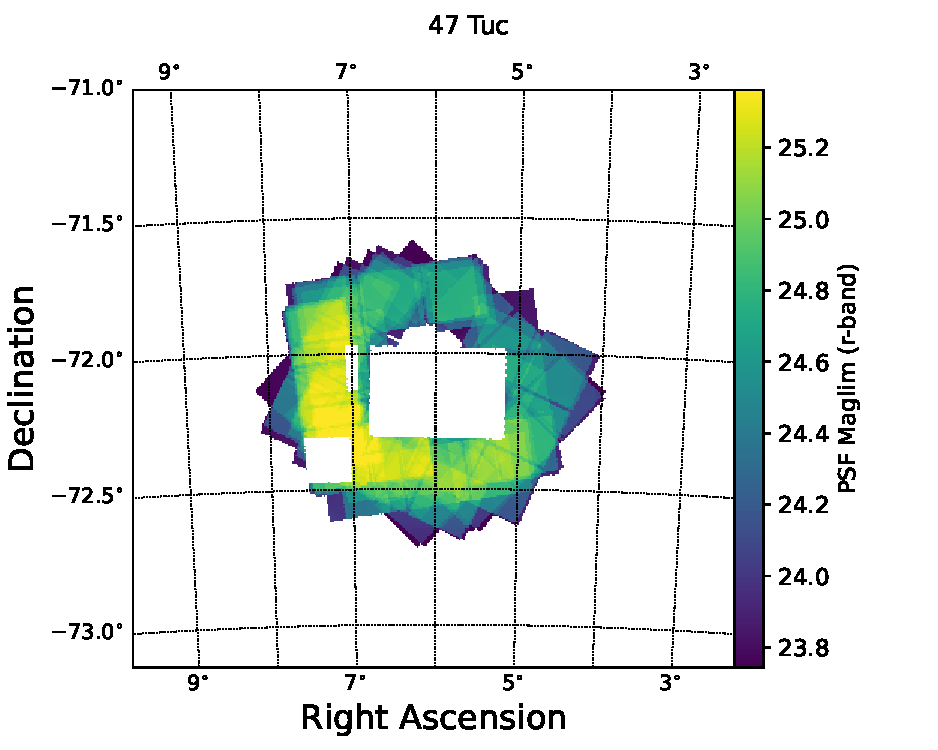
\includegraphics[width=0.33\textwidth]{figures/comcam_psf_maglim_47_tuc_r.pdf}
%        \hspace{1pt}
%        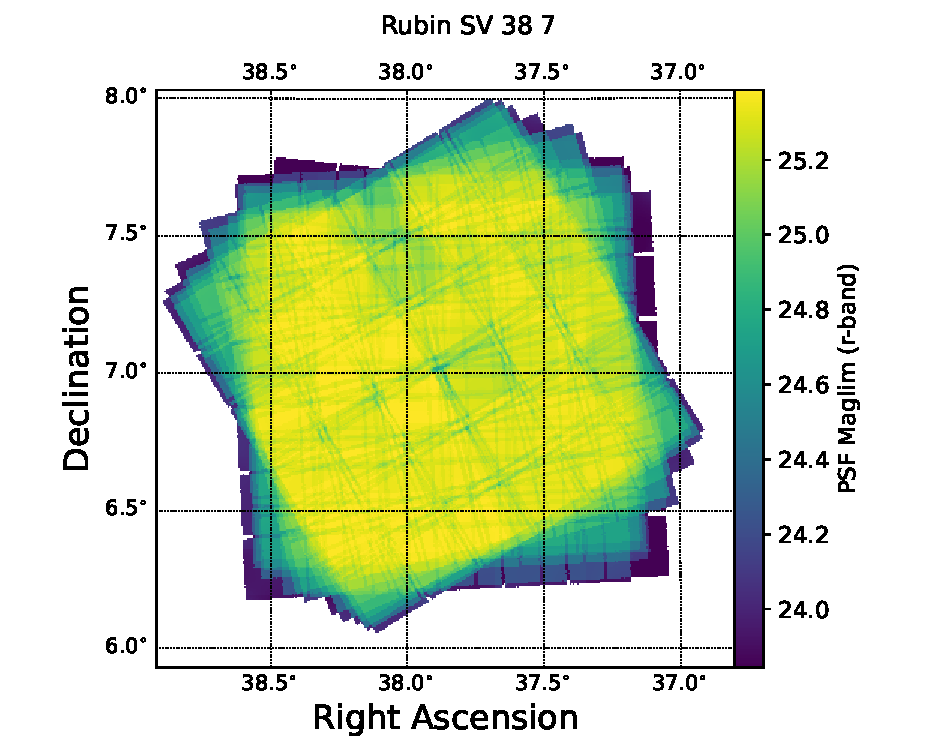
\includegraphics[width=0.33\textwidth]{figures/comcam_psf_maglim_rubin_sv_38_7_r.pdf}
%         \hspace{1pt}
%        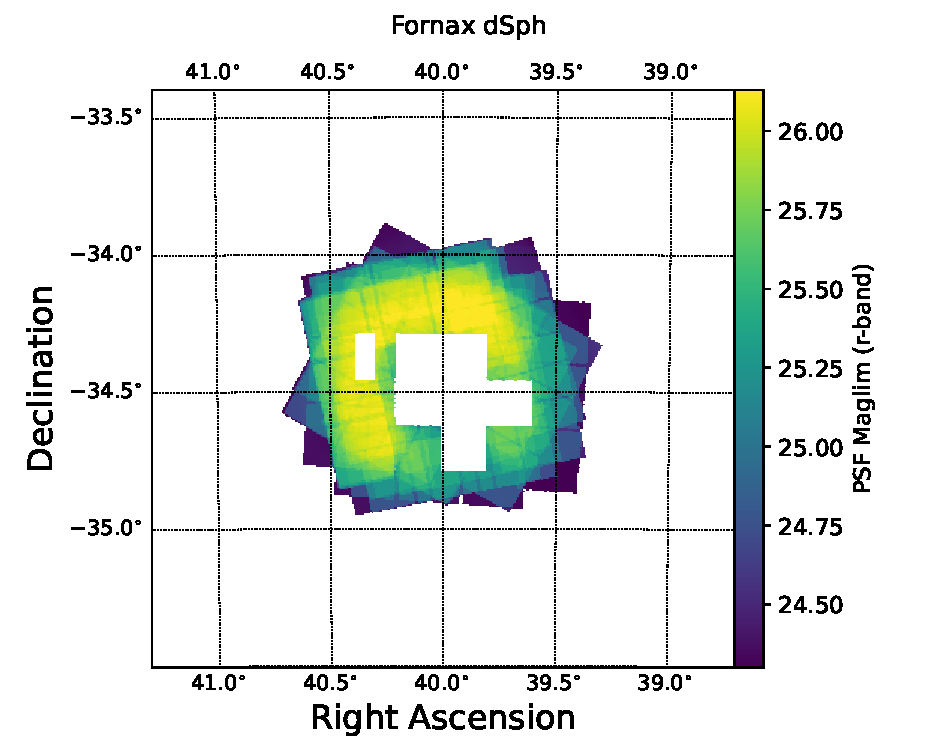
\includegraphics[width=0.33\textwidth]{figures/comcam_psf_maglim_fornax_dsph_r.pdf}
%        \vspace{10pt}
%        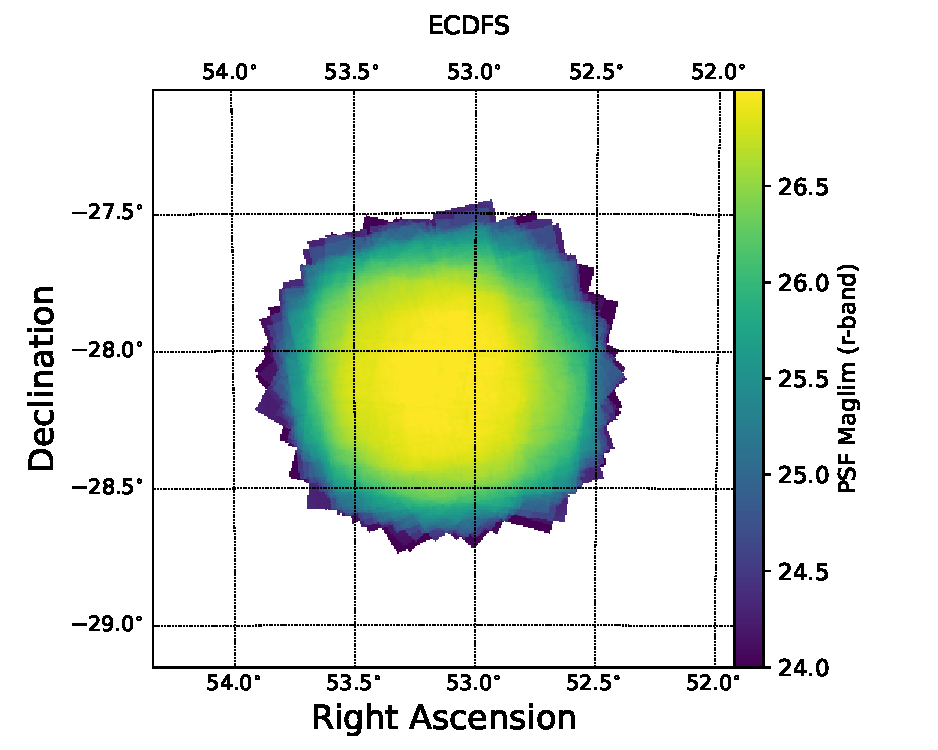
\includegraphics[width=0.32\textwidth]{figures/comcam_psf_maglim_ecdfs_r.pdf}
%        \hspace{1pt}
%        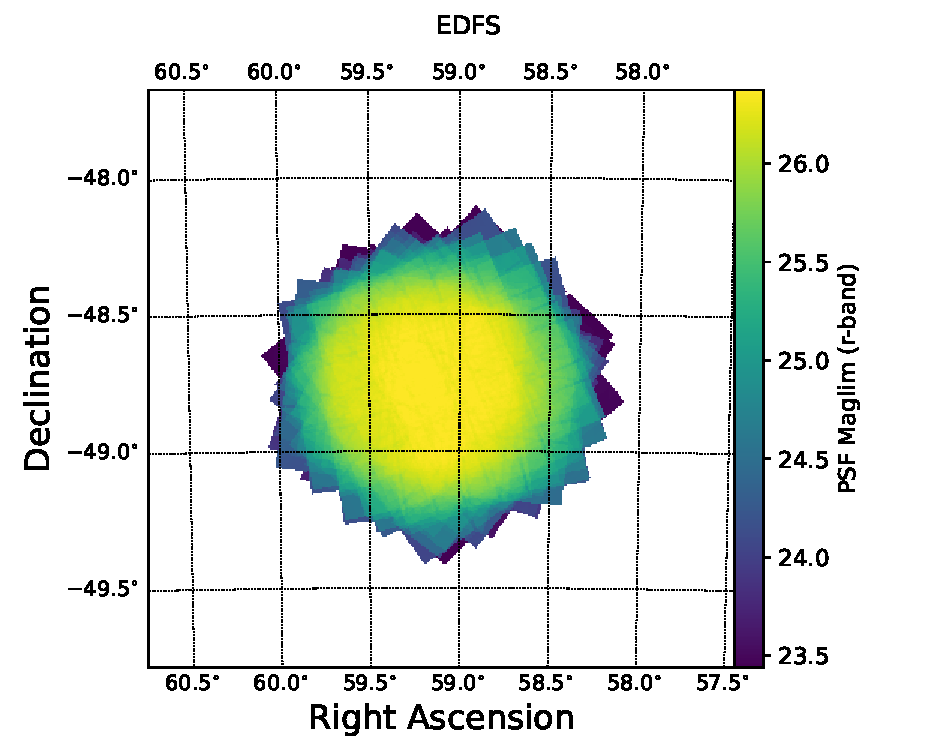
\includegraphics[width=0.32\textwidth]{figures/comcam_psf_maglim_edfs_r.pdf}
%        \hspace{1pt}
%        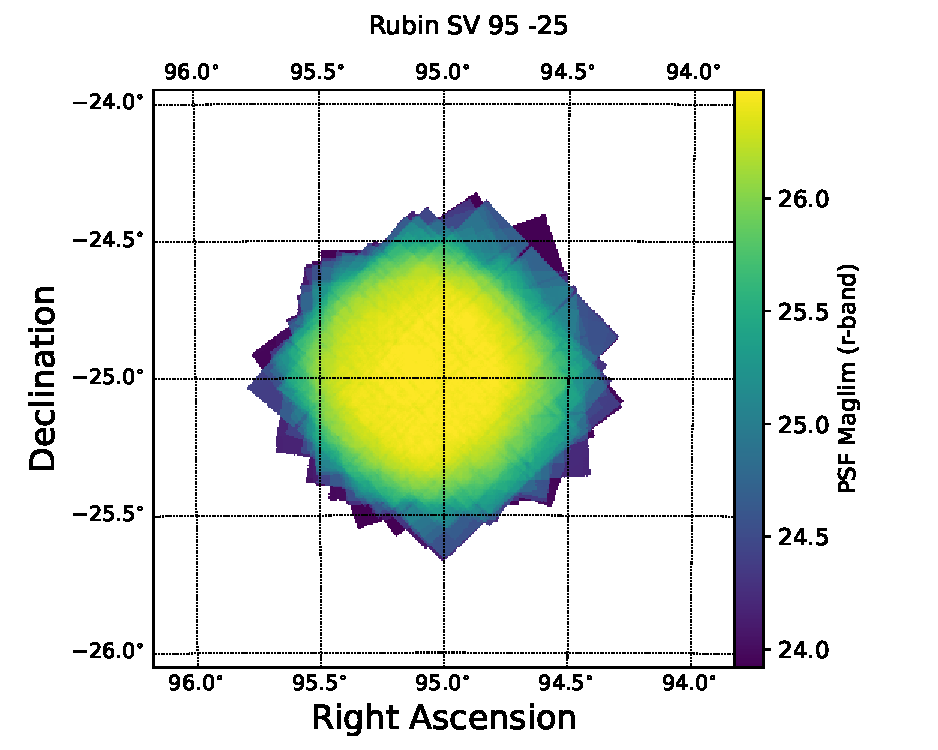
\includegraphics[width=0.32\textwidth]{figures/comcam_psf_maglim_rubin_sv_95_-25_r.pdf}
%        \vspace{10pt}
%        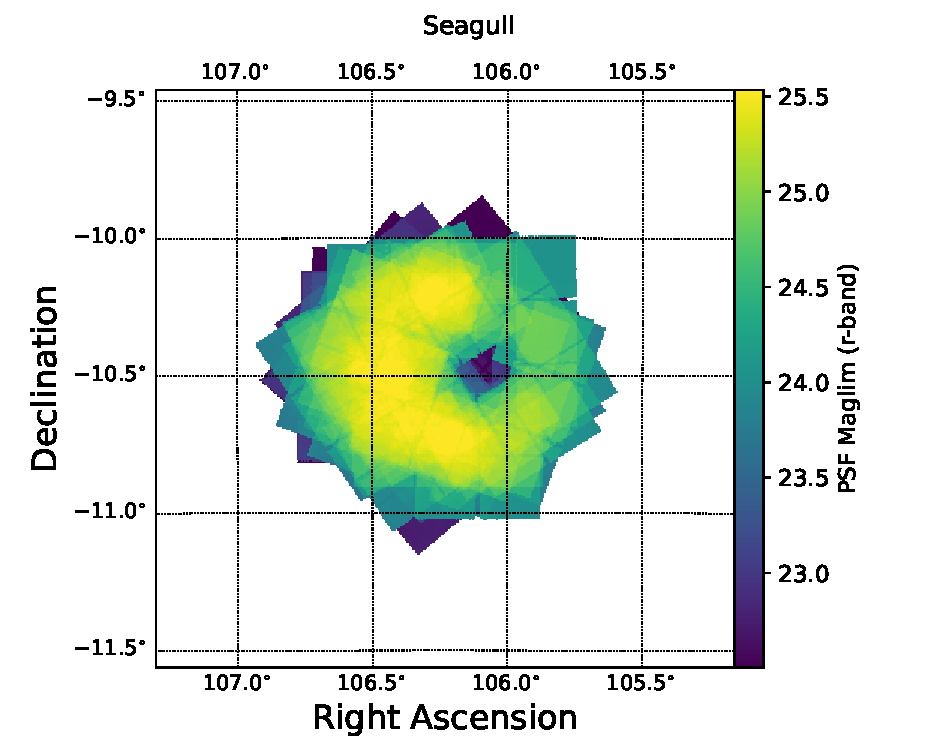
\includegraphics[width=0.32\textwidth]{figures/comcam_psf_maglim_seagull_r.pdf}
%    \end{center}
%    \caption{Cumulative imaging depth expressed in terms of the $S/N=5$ limiting magnitude for unresolved sources for seven ComCam Deep Drilling Fields.
%    First Row (left to right): 47 Tuc, Rubin SV 38 7, Fornax dSph.
%    Second Row (left to right): ECDFS, EDFS, RubinSV 95 -25.
%    Third Row: Seagull.}
%    \label{fig:dp1_fields_psf_maglim}
%\end{figure}

\begin{figure}[htbp]
    \centering
    % First row - 3 images
    \begin{subfigure}[b]{0.3\textwidth}
        \centering
        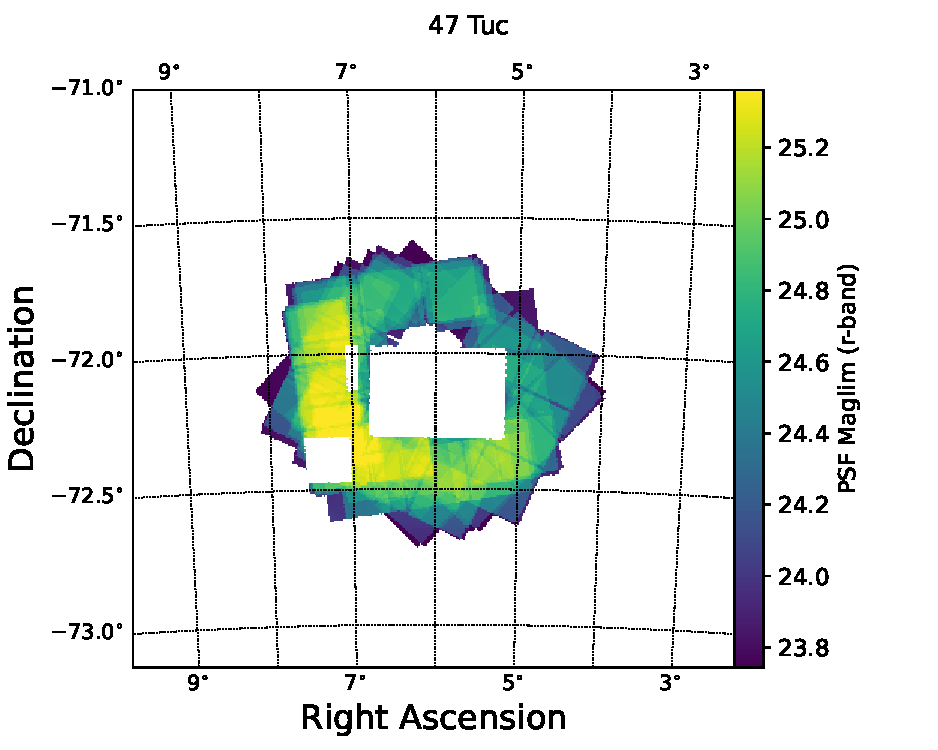
\includegraphics[width=\textwidth]{figures/comcam_psf_maglim_47_tuc_r.pdf}
        \caption{47 Tuc}
        \label{fig:img1}
    \end{subfigure}
    \hfill
    \begin{subfigure}[b]{0.3\textwidth}
        \centering
        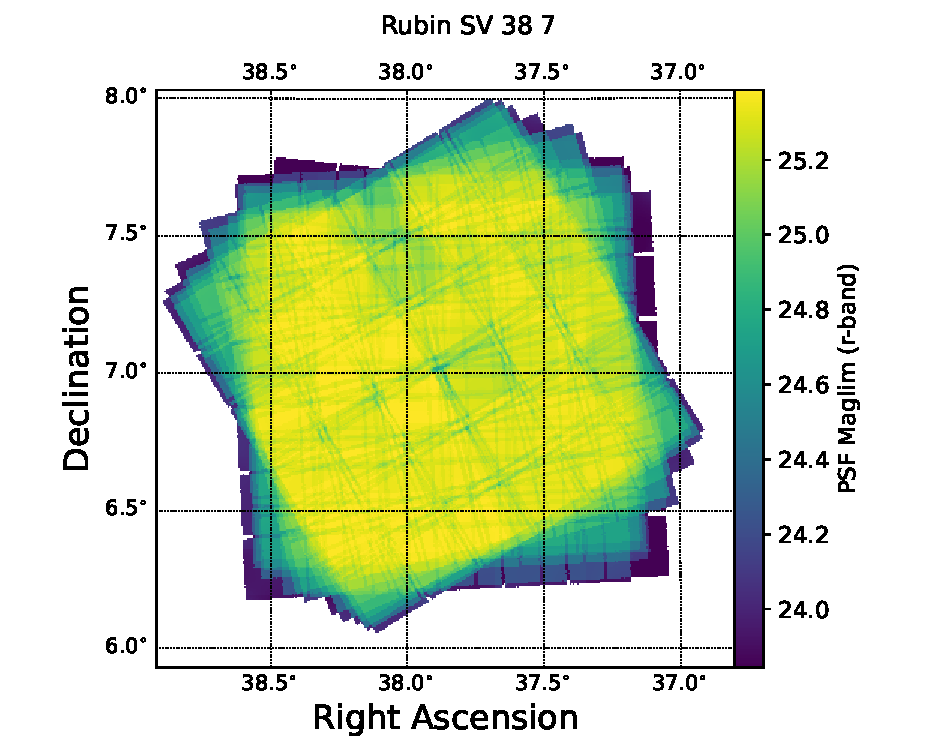
\includegraphics[width=\textwidth]{figures/comcam_psf_maglim_rubin_sv_38_7_r.pdf}
        \caption{Rubin SV 38 7}
        \label{fig:img2}
    \end{subfigure}
    \hfill
    \begin{subfigure}[b]{0.3\textwidth}
        \centering
        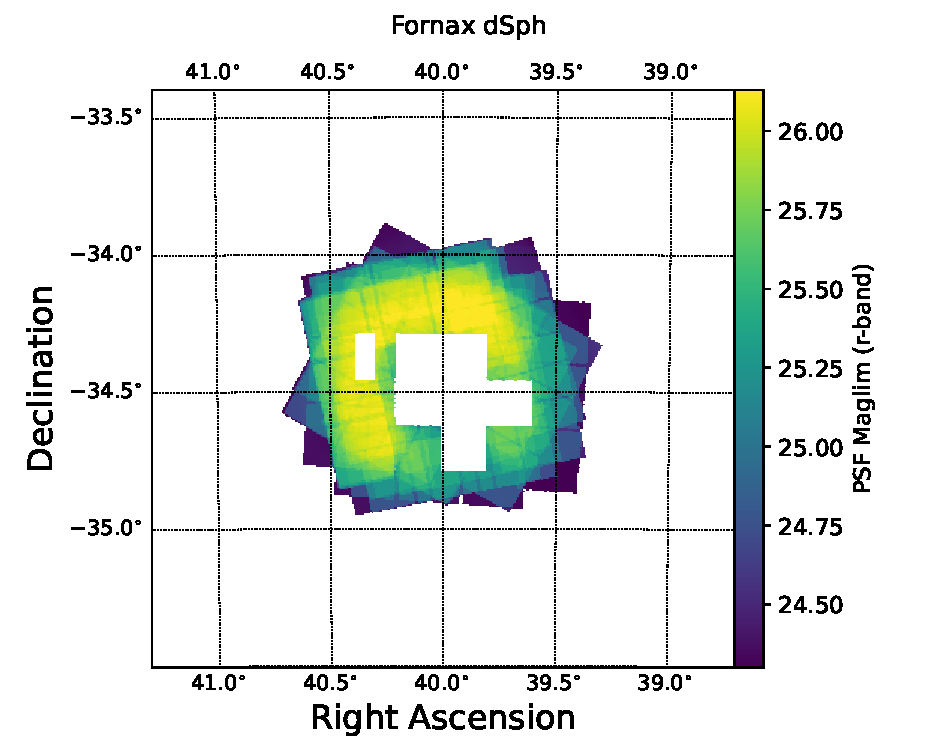
\includegraphics[width=\textwidth]{figures/comcam_psf_maglim_fornax_dsph_r.pdf}
        \caption{Fornax dSph}
        \label{fig:img3}
    \end{subfigure}
    
    \vspace{1em}  % Vertical space between rows
    
    % Second row - 2 images (centered)
    \begin{subfigure}[b]{0.3\textwidth}
        \centering
        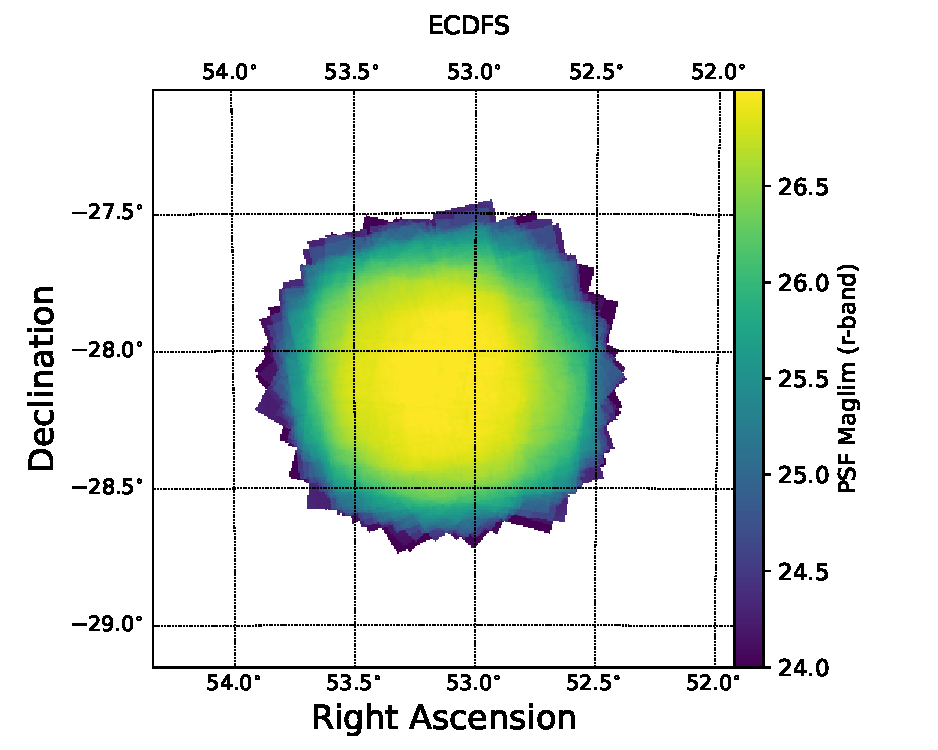
\includegraphics[width=\textwidth]{figures/comcam_psf_maglim_ecdfs_r.pdf}
        \caption{ECDFS}
        \label{fig:img4}
    \end{subfigure}
    \hfill
%    \begin{subfigure}[b]{0.3\textwidth}
%        \centering
%        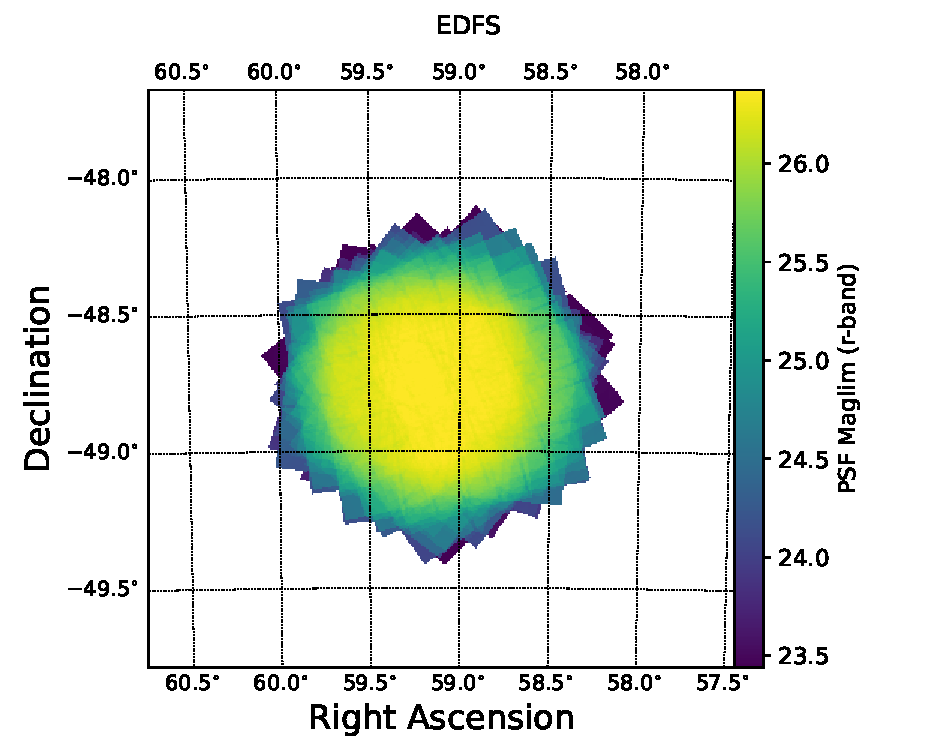
\includegraphics[width=\textwidth]{figures/comcam_psf_maglim_edfs_r.pdf}
%        \caption{EDFS}
%        \label{fig:img5}
%    \end{subfigure}
    
    \vspace{1em}  % Vertical space between rows
    
    % Third row - 3 images
    \begin{subfigure}[b]{0.3\textwidth}
        \centering
        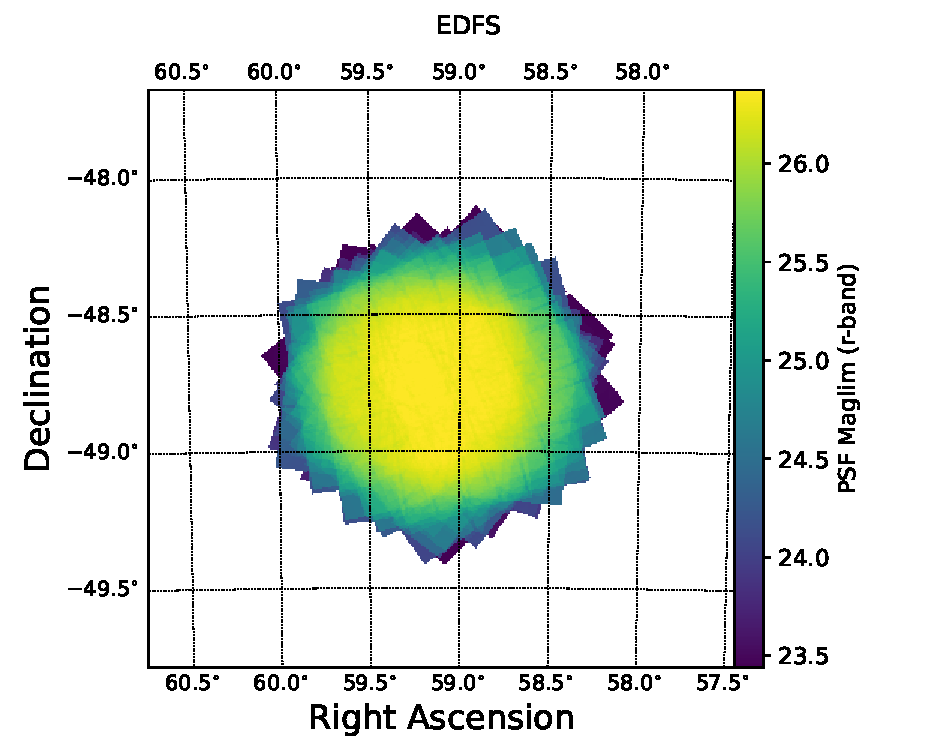
\includegraphics[width=\textwidth]{figures/comcam_psf_maglim_edfs_r.pdf}
        \caption{EDFS}
        \label{fig:img6}
    \end{subfigure}
    \hfill
    \begin{subfigure}[b]{0.3\textwidth}
        \centering
        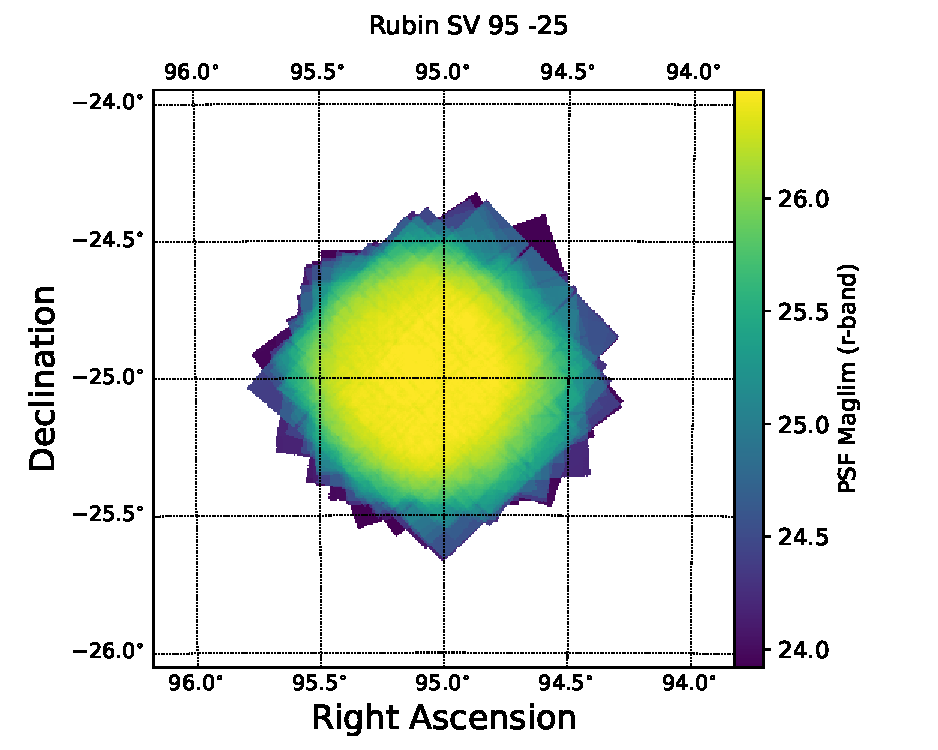
\includegraphics[width=\textwidth]{figures/comcam_psf_maglim_rubin_sv_95_-25_r.pdf}
        \caption{Rubin SV 95 -25}
        \label{fig:img7}
    \end{subfigure}
    \hfill
    \begin{subfigure}[b]{0.3\textwidth}
        \centering
        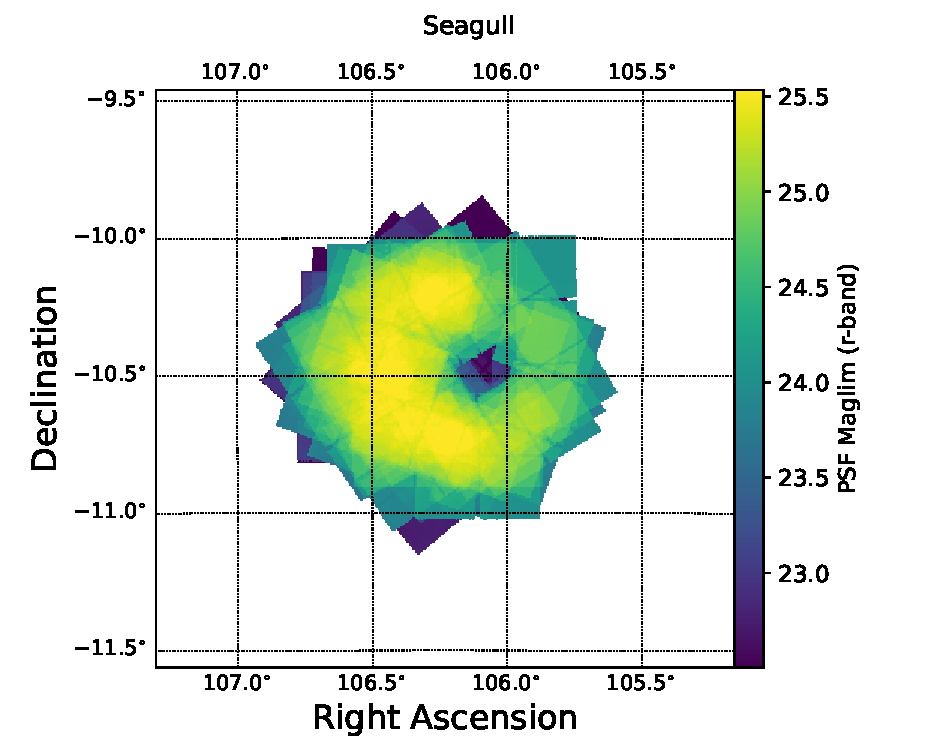
\includegraphics[width=\textwidth]{figures/comcam_psf_maglim_seagull_r.pdf}
        \caption{Seagull}
        \label{fig:img8}
    \end{subfigure}
    
     \caption{Cumulative imaging depth expressed in terms of the $S/N=5$ limiting magnitude for unresolved sources for seven ComCam Deep Drilling Fields.}
     \label{fig:all_images}
\end{figure}

The  processing and preparation of ComCam data for DP1 will take place during the first half of 2025, with an expected DP1 release data in June or July 2025. 
The planned data products for DP1 are presented in table~ \ref{tab:data-preview-summary}. 
Data products that are marked as a stretch goal, DRP ForcedSource Catalogs, Difference Images and DIA Catalogs,  will not be confirmed until close to the DP1 release date. 
DP1 will not contain any DRP  SSP data products in order to focus on readiness for LSSTCam and on providing high quality live LSSTCam SSP Prompt data products as part of the ramp up of Alert Production starting roughly contemporaneously with the DP1 release.


\subsection{Data Preview 2}
\label{sec:dp2}

As the survey begins, all science-grade data collected during the commissioning System Optimization period and subsequent Science Validation Surveys, \S~\ref{sec:commissioning}, is reprocessed to produce the final Data Preview, DP2, which will be released 6 months following the start of operations.

Table~\ref{tab:data-preview-summary} presents a summary of the data products expected in DP2.
DRP Solar System Processing (SSP)  is currently a stretch goal for DP2. 
DRP SSP is intended to be a Rubin-only product; meaning that  It does not start with the catalog from the Minor Planets Center (MPC).


\subsection{Data Release 1}
\label{sec:dr1}

LSST Data Release 1 will be based on the first six months of data taken as part of the 10-year survey. 
Data Release Processing of this dataset is estimated to take six months, making the expected delivery date 1 year following the start of the 10 year survey. 
DR1 will be the first Data Release in which all data products will be provided.

During routine LSST operations, prompt image data products will be made available 80 hours following camera readout. 
They include raw images, processed single visit images (PVIs), difference images, and template images. 
Access to unvetted PVIs and difference images in the first 6 months of the LSST is still to be decided. 
Table~\ref{tab:data-preview-summary} presents a summary of the data products expected in DR1.



